%\documentclass[a4paper,fleqn,longmktitle]{cas-sc}
\documentclass[a4paper,fleqn]{cas-sc}

% \usepackage[numbers]{natbib}
%\usepackage[authoryear]{natbib}
\usepackage[authoryear,longnamesfirst]{natbib}

%%%Author definitions
\def\tsc#1{\csdef{#1}{\textsc{\lowercase{#1}}\xspace}}
\tsc{WGM}
\tsc{QE}
\tsc{EP}
\tsc{PMS}
\tsc{BEC}
\tsc{DE}
%%%
\usepackage{graphicx}
% Uncomment and use as if needed
%\newtheorem{theorem}{Theorem}
%\newtheorem{lemma}[theorem]{Lemma}
%\newdefinition{rmk}{Remark}
%\newproof{pf}{Proof}
%\newproof{pot}{Proof of Theorem \ref{thm}}

\begin{document}
\let\WriteBookmarks\relax
\def\floatpagepagefraction{1}
\def\textpagefraction{.001}

% Short title
\shorttitle{Fine–Coarse Fingerprints of Particulate Matter}

% Short author
\shortauthors{D. Sierra-Porta et~al.}

% Main title of the paper
\title [mode = title]{Fine–Coarse Fingerprints of Particulate Matter in the U.S.: A Land-Use and Seasonal Analysis with Fine Dominance Index}   
% Title footnote mark
% eg: \tnotemark[1]
%\tnotemark[1,2]

% Title footnote 1.
% eg: \tnotetext[1]{Title footnote text}
% \tnotetext[<tnote number>]{<tnote text>} 
%\tnotetext[1]{This document is the results of the researchvproject funded by the National Science Foundation.}

%\tnotetext[2]{The second title footnote which is a longer text mattervto fill through the whole text width and overflow intovanother line in the footnotes area of the first page.}

\author[1]{D. Sierra-Porta}[orcid=0000-0003-3461-1347]
% Corresponding author indication
\cormark[1]
% Email id of the first author
\ead{dporta@utb.edu.co}
%  Credit authorship
\credit{Conceptualization, Methodology, Software, Validation, Formal analysis, Investigation, Resources, Data Curation, Writing - Original Draft, Writing - Review \& Editing, Visualization, Supervision}
\author[1]{Isabella S. Arrieta-Guardo}[orcid=0009-0004-8540-2304]
\credit{Methodology, Software, Formal analysis, Investigation, Data Curation, Writing - Original Draft, Visualization}
\author[1]{Jose F. Gonzalez-Ortiz}[orcid=0009-0009-3380-9504]
\credit{Methodology, Software, Formal analysis, Investigation, Data Curation, Writing - Original Draft, Visualization}
\author[1]{Eduardo A. Negrin-Perez}[orcid=0009-0009-7081-8151]
\credit{Methodology, Software, Formal analysis, Investigation, Data Curation, Writing - Original Draft, Visualization}


% Address/affiliation
\affiliation[1]{organization={Universidad Tecnológica de Bolívar. Escuela de Transformación Digital.},
                addressline={Parque Industrial y Tecnológico Carlos Vélez Pombo Km 1 Vía Turbaco.},
                city={Cartagena de Indias},
                postcode={130010},
                country={Colombia}}
                
% Corresponding author text
\cortext[cor1]{Corresponding author}
%\cortext[cor2]{Principal corresponding author}

% Footnote text
%\fntext[fn1]{This is the first author footnote. but is common to third author as well.}
%\fntext[fn2]{Another author footnote, this is a very long footnote and it should be a really long footnote. But this footnote is not yet sufficiently long enough to make two lines of footnote text.}

% For a title note without a number/mark
%\nonumnote{This note has no numbers. In this work we demonstrate $a_b$ the formation Y\_1 of a new type of polariton on the interface between a cuprous oxide slab and a polystyrene micro-sphere placed on the slab.}

% Here goes the abstract
\begin{abstract}
Air pollution mixtures vary across space, seasons, and land uses, challenging source-informed assessment with a single particulate ratio. Using publicly available EPA AirData (2022–2024), we analyze daily PM$_{2.5}$ and PM$_{10}$ at 171 monitors that met a $\ge$1000-day completeness screen and are stratified by land use (commercial, residential, industrial, agricultural, desert, military reservation, forest) and location setting (urban and center city, suburban, rural). We introduce a sample-level Fine Dominance Index (FDI) derived from PM$_{2.5}$ and PM$_{10}$ and summarize distributions by season (winter, spring, summer, autumn). To compare contexts, we aggregate cell-wise (land use $\times$ location setting $\times$ season) and construct a standardized composite index (IFS) from FDI and distributional descriptors, alongside nonparametric contrasts (Kruskal--Wallis with Holm-adjusted Mann--Whitney post hoc tests) and effect sizes (Cliff’s $\delta$). Uncertainty for cell means is quantified with bootstrap 95\% intervals.

Results show clear heterogeneity across land uses within the same setting and season. Fine-dominant hotspots concentrate in winter for built environments (commercial, residential, industrial), consistent with shallow boundary layers and heating/traffic influences, whereas coldspots cluster in desert settings---especially rural---indicating persistent coarse dust. Findings are robust to alternative IFS weightings and completeness thresholds, with rank changes confined to mid-tier cells. Practically, the framework supports season- and context-specific management: wintertime controls in built environments and coarse-dust abatement where desert influence prevails. Because it relies only on routinely reported PM$_{2.5}$ and PM$_{10}$, the approach is scalable and reproducible, and it highlights where more detailed chemical measurements would be most informative.
\end{abstract}

% Use if graphical abstract is present
% \begin{graphicalabstract}
% \includegraphics{figs/grabs.pdf}
% \end{graphicalabstract}

% Research highlights
\begin{highlights}
\item FDI (sample) and IFS (cell) classify fine vs coarse dominance across U.S. sites.
\item Winter hotspots in built environments; desert rural cells are persistent coldspots.
\item Nonparametric tests and bootstrap CIs yield robust, scalable, policy-ready screening.
\end{highlights}

% Keywords
% Each keyword is seperated by \sep
\begin{keywords}
EPA AirData \sep PM$_{2.5}$ \sep PM$_{10}$ \sep particulate matter \sep Fine Dominance Index (FDI) \sep composite index \sep land use \sep 
urbanicity \sep seasonality \sep nonparametric tests
\end{keywords}


\maketitle
\section{Introduction}
Air pollution remains a critical environmental and public health concern in the United States and worldwide. Its complexity arises from the interplay among emission sources, land-use patterns, and meteorology, which together shape the spatial and temporal variability observed at monitoring networks. The U.S. Environmental Protection Agency (EPA) operates reference stations that track key criteria pollutants, including particulate matter with aerodynamic diameters below 10\,\textmu m (PM$_{10}$) and 2.5\,\textmu m (PM$_{2.5}$), across diverse settings such as urban cores, suburban belts, and rural areas, and across land-use contexts including commercial, residential, industrial, agricultural, desert, military reservations, and forests.

A growing body of research shows that disaggregating observations by location and land use improves inference on dominant sources and exposure disparities \citep{Kilpatrick2024, Hart2009, Sooktawee2020}. Agricultural regions contribute substantial ammonia that promotes secondary PM$_{2.5}$ formation and exhibits rising NH$_3$ trends in connection with confined animal feeding operations \citep{Burns2023, Ogwu2024}. Urban corridors are persistently influenced by traffic-related emissions \citep{Alvarado-Molina2023, Nasr2025}, while industrial and residential zones display distinct particulate and gaseous profiles \citep{Bikis2023, Roy2023}.

Seasonal cycles further modulate concentrations via boundary-layer dynamics, heating, photochemistry, wildfires, and dust intrusions that can episodically elevate particulate levels across large regions \citep{Achilleos2020, Allajbeu2017, Velsquez-Garca2024, Rawat2024, Butler2024, Yu2021}. In parallel, the increasing availability of regulatory-grade monitors and complementary low-cost sensors has enhanced spatial coverage and temporal resolution, albeit with calibration and comparability challenges \citep{Chen2022, Brilli2021}.

A common approach to characterizing the fine–coarse partition relies on the PM$_{2.5}$/PM$_{10}$ ratio, typically higher in combustion- and traffic-influenced environments and lower where resuspension or natural dust dominates \citep{Fan2021, Colangeli2022}. While informative, single-ratio summaries and fixed thresholds can mask heterogeneity across land uses and along urban–suburban–rural gradients, where long-term patterns and disparities also emerge \citep{Kilpatrick2024, Liu2023, Jbaily2022}. These considerations motivate compact, interpretable indices built from PM$_{10}$ and PM$_{2.5}$, together with distributional descriptors, to derive fingerprints of source dominance that are comparable across settings and seasons.

In this study, we analyze EPA observations stratified by land use and urbanicity and conduct a seasonal assessment using climatological definitions. We introduce two complementary summaries that we use throughout: a sample-level Fine Dominance Index (FDI), designed to increase with the predominance of fine particles, and a cell-level composite score (IFS) that standardizes multiple cell summaries into a single, comparable fingerprint across land uses and seasons. Detailed constructions are provided in the Methods, but the roles are simple: FDI provides physically interpretable, per-sample information; IFS provides a standardized ranking at the land use–location–season cell level. Beyond averages, we contrast entire distributions using nonparametric omnibus tests with multiplicity-controlled post hoc comparisons and effect sizes, and we identify seasonal hotspots and coldspots using bootstrap intervals for cell means. The framework yields a concise, reproducible fingerprint of particulate dominance that supports source-informed air-quality assessment across heterogeneous U.S. environments.

Our scope is intentionally complementary to chemically speciated source apportionment. By relying on routinely reported PM$_{10}$ and PM$_{2.5}$, the proposed indices and distributional contrasts can be applied at scale without additional instrumentation. This practicality comes with limitations: ratio-based fingerprints are indirect, can be sensitive to measurement artifacts and denominator effects, and do not by themselves separate individual sources. We mitigate these concerns by combining multiple derived indices with distributional shape descriptors, by stratifying analyses by land use and urbanicity, and by reporting uncertainty via bootstrap intervals and nonparametric tests. The resulting evidence is well suited to screening, prioritization, and policy design where rapid, interpretable comparisons across settings and seasons are needed, and it can guide where more detailed chemical measurements would be most informative.

The remainder of this article is organized as follows. The next section describes data sources, quality-control steps, seasonal definitions, and the construction of the derived indices and statistical tests. We then present distributional results and hotspot/coldspot maps by land use, location setting, and season, followed by sensitivity and robustness checks. We close with implications for monitoring and management and with directions for integrating these fingerprints with chemically resolved source apportionment.

\section{Data and methods}
\subsection{Data}

We used pre-generated daily summary files from the EPA AirData (AQS) portal for 2022--2024 covering fine particulate matter (PM$_{2.5}$), inhalable particles (PM$_{10}$), and coarse particulate matter (PM$_{c}$). Specifically, we downloaded the daily archives for PM$_{2.5}$ FRM/FEM mass (parameter code 88101; \texttt{daily\_88101\_YYYY.zip}), PM$_{2.5}$ non-FRM/FEM mass (88502; \texttt{daily\_88502\_YYYY.zip}), PM$_{10}$ mass (81102; \texttt{daily\_81102\_YYYY.zip}), and PM$_{c}$ (86101; \texttt{daily\_86101\_YYYY.zip}) from the AirData download page (\url{https://aqs.epa.gov/aqsweb/airdata/download_files.html}). Each file provides one daily aggregate per monitor and parameter (the \textit{Arithmetic Mean} of valid sub-daily measurements) together with site metadata, geolocation, land-use class, and location setting.

For each parameter, we concatenated the 2022, 2023, and 2024 archives, retained the minimal fields needed for stratification (local date, daily mean, latitude/longitude, land-use, and location setting), removed ancillary fields not used downstream (e.g., method codes and textual addresses), and dropped duplicate rows that occasionally arise from file updates. We then harmonized land-use labels across years and retained the three AQS location-setting categories used throughout: Urban and center city, Suburban, and Rural. Parameter-specific tables were merged by monitor and date to enable computation of derived ratios. In this study, PM$_{10}$ and PM$_{2.5}$ FRM/FEM is treated as the primary regulatory series for analysis; PM$_{2.5}$ non-FRM/FEM is used as a complementary series for sensitivity checks; PM$_{c}$ is used only for coarse-fraction consistency checks.

\subsubsection*{Network composition and completeness}

The monitoring network spans a wide range of land uses and urbanicity. Table~\ref{tab:stations_counts} summarizes counts by land-use category and by location setting in our raw inventory (as reported in AQS metadata).

\begin{table}[htb]
\centering
\caption{Station counts in the raw inventory (as reported in AQS metadata).}
\label{tab:stations_counts}
\begin{minipage}{0.48\linewidth}
\centering
\begin{tabular}{lr}
\hline
\textbf{Land use} & \textbf{Count} \\
\hline
Residential & 1645 \\
Commercial & 1099 \\
Industrial & 725 \\
Agricultural & 602 \\
Forest & 437 \\
Desert & 105 \\
Military reservation & 13 \\
Mobile & 69 \\
Blighted areas & 3 \\
Unknown & 21 \\
\hline
\end{tabular}
\end{minipage}\hfill
\begin{minipage}{0.48\linewidth}
\centering
\begin{tabular}{lr}
\hline
\textbf{Location setting} & \textbf{Count} \\
\hline
Rural & 1851 \\
Suburban & 1615 \\
Urban and center city & 1251 \\
Unknown & 13 \\
\hline
\end{tabular}
\end{minipage}
\end{table}

Because many monitors exhibit intermittent reporting, we applied a completeness screen at the \textit{station--parameter} level. For each station and parameter we counted non-missing daily means over 2022--2024 and retained stations with at least 1000 valid days (approximately $1000/(365\times 3)\approx 91.3\%$ coverage). For ratio-based metrics (e.g., PM$_{2.5}$/PM$_{10}$ and derivatives), daily computations required same-day availability of both PM$_{2.5}$ and PM$_{10}$; days lacking either measurement were excluded from ratio calculations. We also removed invalid/undefined values (e.g., zero or negative denominators, infinities, explicit missing codes) and harmonized land-use and location-setting labels across years. Unless noted otherwise, downstream inferential analyses focus on the main land-use classes with substantive sample sizes (commercial, residential, industrial, agricultural, desert, military reservation, forest) and exclude \textit{mobile}, \textit{blighted areas}, and \textit{unknown} categories due to low counts or ambiguous interpretation (the retained network may still contain a few such sites for mapping completeness).

After applying the completeness screen, the analytical sample comprises \textbf{171} monitors distributed across the main land-use classes and across the urban--suburban--rural gradient. Table~\ref{tab:retained_counts} summarizes the cross-classification by land use and location setting, and Figure~\ref{fig:stations_map} shows the geospatial distribution of retained sites, colored by land use.

\begin{figure}[htb]
 \centering
 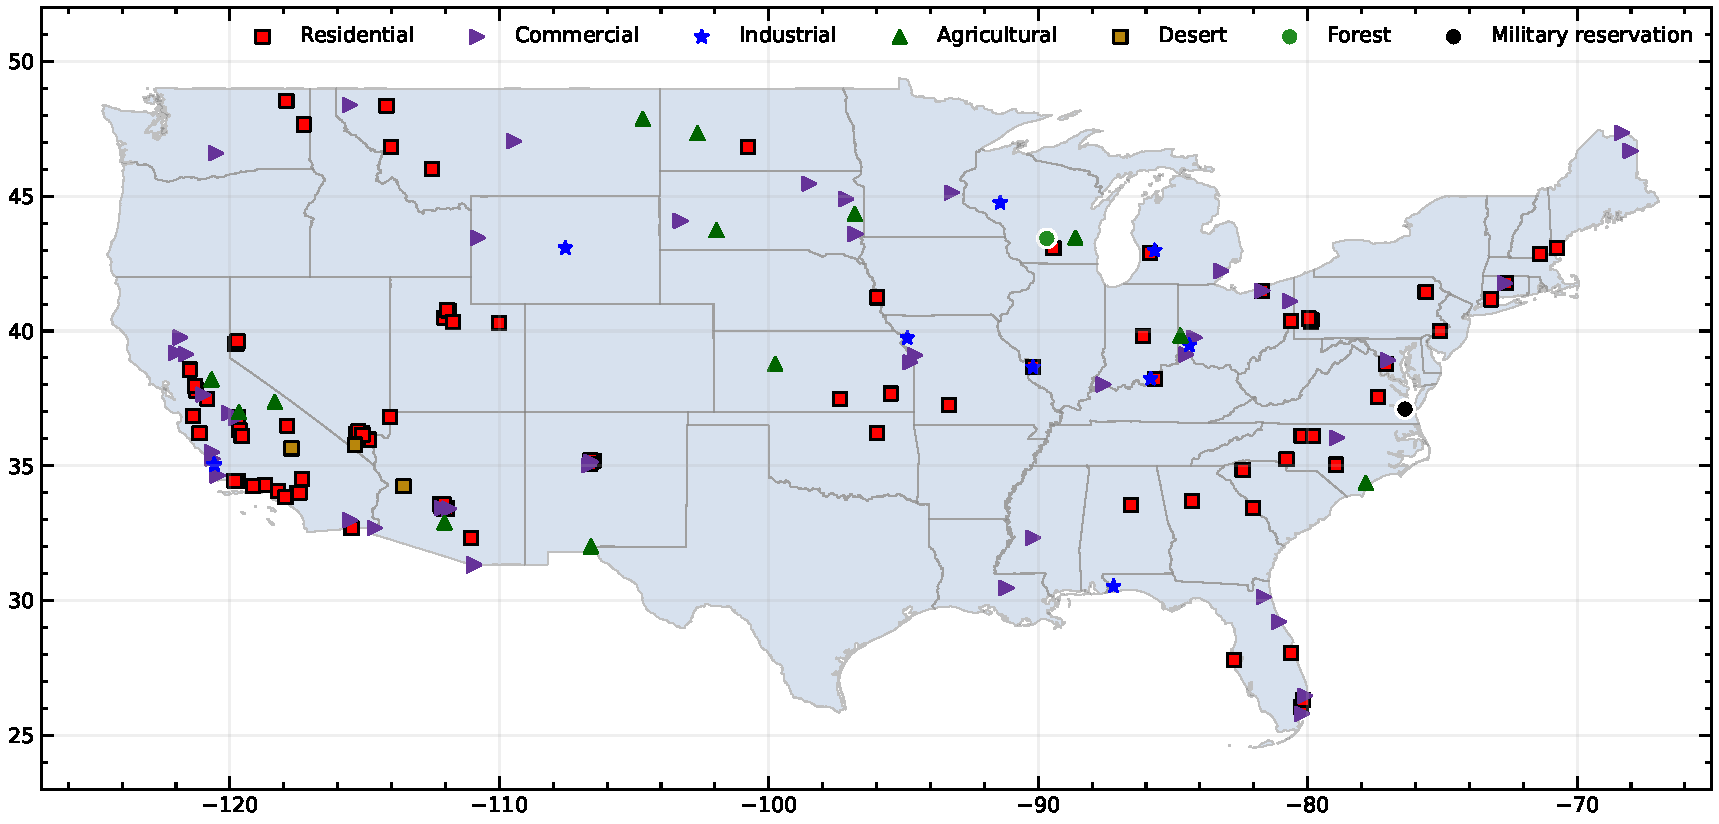
\includegraphics[width=\linewidth]{Stations.pdf}
 \caption{Geolocated map of retained stations ($n=171$) after applying the completeness screen ($\geq 1000$ valid daily values, 2022--2024). Colors denote land-use classes.}
 \label{fig:stations_map}
\end{figure}

\begin{table}[htb]
\centering
\caption{Retained stations by land use and location setting ($n=171$).}
\label{tab:retained_counts}
\begin{tabular}{l l r}
\toprule
\textbf{Land Use} & \textbf{Location Setting} & \textbf{Count} \\
\midrule
Residential & Suburban & 56 \\
Residential & Urban and center city & 32 \\
Commercial  & Urban and center city & 27 \\
Commercial  & Suburban & 16 \\
Agricultural & Rural & 13 \\
Residential & Rural & 5  \\
Industrial  & Suburban & 4  \\
Commercial  & Rural & 3  \\
Industrial  & Rural & 3  \\
Industrial  & Urban and center city & 3  \\
Desert   & Rural & 2  \\
Mobile   & Suburban & 2  \\
Mobile   & Urban and center city & 2  \\
Desert   & Urban and center city & 1  \\
Forest   & Rural & 1  \\
Military reservation & Suburban & 1  \\
\midrule
\multicolumn{2}{r}{\textbf{Total}} & \textbf{171} \\
\bottomrule
\end{tabular}
\end{table}

\subsection{Methods}

We defined climatological seasons based on calendar months: Winter (December--February), Spring (March--May), Summer (June--August), and Autumn (September--November). Each daily record inherits the season label from its date; summaries and tests are executed seasonally unless stated otherwise.

We constructed three ratios that capture complementary aspects of the fine--coarse partition \citep{Fan2021}:
\begin{equation}
r_{12}=\frac{\mathrm{PM}_{2.5}}{\mathrm{PM}_{10}},\qquad
r_{21}=\frac{\mathrm{PM}_{10}}{\mathrm{PM}_{2.5}},\qquad
r_{0}=\frac{\mathrm{PM}_{10}-\mathrm{PM}_{2.5}}{\mathrm{PM}_{10}+\mathrm{PM}_{2.5}}\,,
\end{equation}
together with a per-sample Fine Dominance Index (FDI),
\begin{equation}
\mathrm{FDI}=\frac{\mathrm{PM}_{2.5}}{\mathrm{PM}_{10}}\,(1-r_{0})\,,
\end{equation}
designed to increase with fine-particle dominance. Ratios were computed only when denominators were strictly positive; infinite results were treated as missing. These per-sample quantities support distributional contrasts (e.g., violin/box plots) and nonparametric tests.

For interpretability across contexts, we summarize observations in “cells” defined by the cross of Land Use, Location Setting, and Season. Within each cell we compute distributional descriptors for $r_{0}$ and FDI: mean, standard deviation, skewness, and kurtosis (Fisher definition). To provide a single fingerprint per cell, we build a composite index IFS from standardized features,
\begin{equation}
\mathrm{IFS} \;=\; w_{\mathrm{FDI}}\;z\!\big(\overline{\mathrm{FDI}}\big)
 \;+\; w_{r_0}\;z\!\big(\overline{r_{0}}\big)
 \;+\; w_{\mathrm{skew}}\;z\!\big(\mathrm{skew}(r_{0})\big)
 \;+\; w_{\mathrm{kurt}}\;z\!\big(\mathrm{kurt}(r_{0})\big)\,,
\end{equation}
where $z(\cdot)$ denotes cross-cell $z$-scores. We use $w_{\mathrm{FDI}}=1.5$, $w_{r_0}=-1.0$, $w_{\mathrm{skew}}=0.5$, and $w_{\mathrm{kurt}}=0.5$. The weighting emphasizes fine dominance via $\overline{\mathrm{FDI}}$, penalizes coarse dominance via $\overline{r_0}$, and assigns modest influence to tail behavior via skewness/kurtosis (used as shape regularizers rather than drivers of the ranking). We corroborate the a priori weighting by comparing IFS with the first principal component of the standardized feature set and by a weight-sensitivity analysis (grids over plausible weights) using Kendall’s $\tau$ rank correlation.

Because components are standardized across cells, IFS is on a $z$-scale: values near 0 reflect network-average behavior; $\pm 1$ represent roughly one standard deviation above/below the network average. Higher IFS values indicate stronger fine-particle dominance with relatively muted coarse bursts, whereas lower values indicate coarse-dust influence and episodic tail behavior. Thin cells (small $n$ or large uncertainty) are flagged and interpreted with caution.

For each cell we estimate a 95\% confidence interval for the \textbf{mean FDI} by nonparametric bootstrap with $B=1000$ resamples of the daily values contributing to that cell; we also report the number of contributing days $n$. Cells are flagged as thin when $n<300$ or when the two-sided 95\% interval for $\overline{\mathrm{FDI}}$ exceeds a prespecified tolerance (we used 0.10 FDI units); flagged cells are visually muted and excluded from “top/bottom” league tables.

To compare land uses without assuming normality, we apply Kruskal--Wallis omnibus tests \citep{Lachenbruch1991, MacFarland2016} within each Location Setting $\times$ Season for the following per-sample metrics: FDI, $r_{0}$, $r_{12}$, $r_{21}$, PM$_{2.5}$, and PM$_{10}$. Pairwise post hoc contrasts use two-sided Mann--Whitney tests \citep{Nasr2025, Grzegorzewski2018} with Holm correction for multiple comparisons. We report effect sizes using Cliff’s delta \citep{Kala2024, Meissel2024} and classify magnitudes using conventional thresholds (approximately 0.15 small, 0.33 medium, 0.47 large). Groups with fewer than 20 daily observations are omitted from a given test to avoid unstable ranks.

Visualization follows two complementary views. We present faceted heatmaps of IFS by Land Use (rows) and Season (columns) stratified by Location Setting, using a common, zero-centered color scale; cells with insufficient information are muted, and $n$ and bootstrap intervals are reported in tables. Distributional shapes are displayed with violin and box plots of FDI using common $y$-axes across facets. For visualization only, and never for hypothesis testing, we optionally winsorize FDI at the 1st--99th percentiles to prevent extreme outliers from compressing axis scales; all inferential procedures use the raw filtered data.

All analyses were performed in Python using \texttt{pandas}, \texttt{numpy}, \texttt{scipy}, \texttt{matplotlib}/\texttt{seaborn}, and \texttt{scikit-learn}. Code reproduces the screening criteria, derived-variable construction, and statistical tests described above using publicly available EPA AirData files for 2022--2024 (\url{https://aqs.epa.gov/aqsweb/airdata/download_files.html}).



\section{Results and Discussion}
\subsection{Sample-level distributions of fine dominance}

Starting from the retained daily records, we first characterize variability at the sample level with the Fine Dominance Index (FDI) across land-use classes, location settings, and seasons. Figure~\ref{fig:fdi_facets} displays faceted boxplots under a common $y$-axis, enabling like-for-like comparisons without rescaling.

\begin{figure}[htb]
  \centering
  \includegraphics[width=\linewidth]{fig2_fdi_box_facets.png}
  \caption{Sample-level Fine Dominance Index (FDI) by land use with facets for location setting (rows) and season (columns). Boxes show medians and interquartile ranges with a common $y$-axis; whiskers span the 5th–95th percentiles and outliers are hidden for clarity. Larger FDI indicates stronger fine-particle dominance relative to coarse contributions.}
  \label{fig:fdi_facets}
\end{figure}

The facets reveal clear heterogeneity across land uses within the same setting and season, with visibly separated medians and interquartile ranges in several comparisons and broader tails where episodic coarse contributions are more likely. For visualization only, extreme tails may be winsorized as noted in the Methods; all inference uses the raw filtered data.

These patterns align with the physical interpretation of FDI: higher values point to combustion- and traffic-related influence, whereas lower values indicate coarse-dust dominance from resuspension or natural dust \citep{Liu2023, Xu2020}. Within a given location setting, contrasts between commercial/industrial versus agricultural/desert classes plausibly reflect activity patterns and surface characteristics \citep{Wei2021, Clark2013}. Seasonally, the compression or widening of distributions is consistent with boundary-layer dynamics, heating-related emissions, photochemistry, and dust or smoke episodes. Where distributions overlap, the overlap suggests mixed-source environments or within-class heterogeneity; conversely, well-separated quartiles point to distinct source regimes that motivate formal testing.

Outlier-prone tails in specific land-use–season cells typically coincide with episodic coarse events (negative excursions in FDI), localized construction or road dust, or short bursts of intense combustion (positive excursions). These tails are informative for exposure assessment but can obscure central tendencies in low-$n$ cells; hence the completeness screen and the complementary, cell-wise summaries presented next. Overall, Figure~\ref{fig:fdi_facets} frames the composite fingerprints and hypothesis tests by indicating where separations are strongest, where overlap persists, and where seasonal modulation is most pronounced.

\subsection{Cell-wise seasonal fingerprints (IFS)}

Building on the sample-level view, we next summarize conditions at the cell level (Land Use $\times$ Location Setting $\times$ Season) using the composite, standardized index IFS. Figure~\ref{fig:fdi_heatmaps} displays seasonal heatmaps in three panels (one per location setting) under a common, zero-centered color scale to enable like-for-like comparisons; cells with insufficient information are muted.

The patterns reinforce and sharpen the distributional view. In rural contexts, winter shows clear fine-dominance hotspots for commercial, residential, industrial, and forest classes, consistent with shallow boundary layers and heating-related emissions, whereas desert cells remain negative across seasons, indicating coarse-dust influence \citep{Jandacka2024, Yu2021, Czernecki2021}. Suburban areas exhibit positive winter and summer cells for several built environments—notably residential—while agricultural and desert cells are lower or mixed depending on the season \citep{Bell2007, Burns2023}. In urban and center-city settings, spring and especially summer highlight fine-dominant cells for residential and commercial land uses, plausibly reflecting traffic and warm-season combustion/photochemistry, whereas desert cells are consistently negative, with the strongest coarse signature in spring and autumn \citep{Clements2016}. These contrasts align with the interpretation of IFS (higher values indicate stronger fine-particle dominance relative to the network average for that season).

Two practical points guide interpretation. First, because IFS is standardized and centered at zero, positive cells mark regimes that are more fine-dominated than the network average for that season, while negative cells indicate relatively coarse-dominated regimes. Second, apparent outliers often correspond to episodic dust or smoke seasons; when contributing sample sizes are small or bootstrap uncertainty for the mean FDI is wide, such cells should be treated cautiously and are muted in the figure. Overall, the heatmaps identify robust seasonal hotspots and coldspots that motivate the formal nonparametric contrasts presented next.

\begin{figure}[htb]
  \centering
  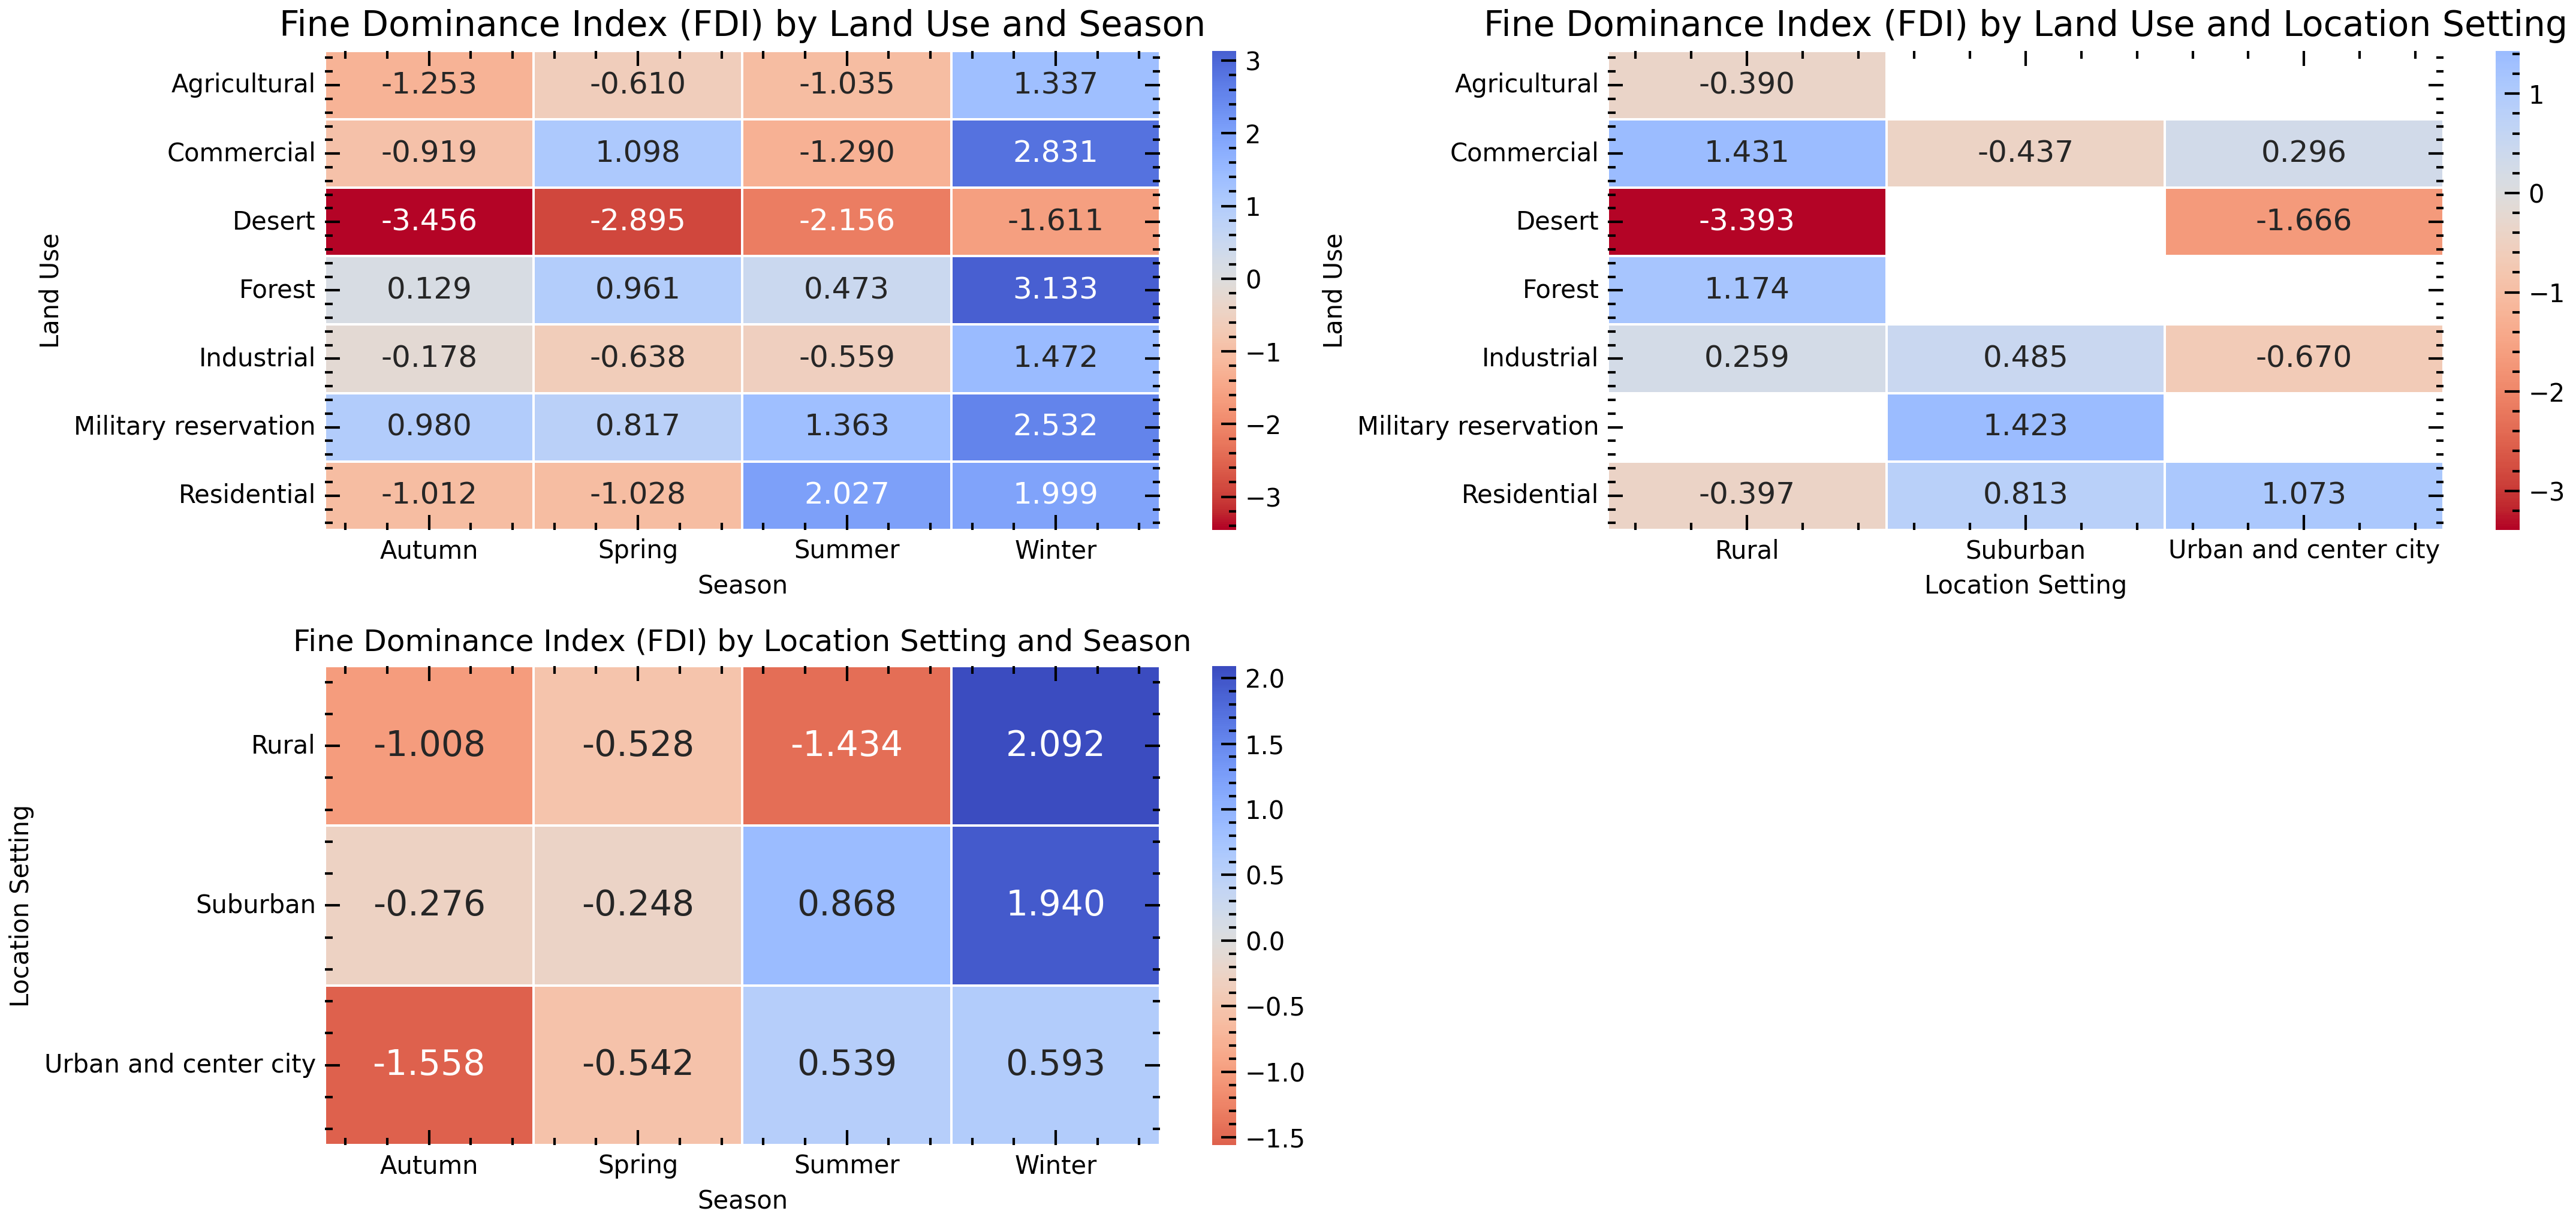
\includegraphics[width=\linewidth]{fig1_fdi_heatmap.png}
  \caption{Cell-wise seasonal fingerprints using the standardized composite index (IFS) by land use (rows) and season (columns), stratified by location setting (three panels). The color scale is centered at zero to enable cross-panel comparison; muted cells denote insufficient information. Positive values indicate stronger fine-particle dominance relative to the network average for the corresponding season.}
  \label{fig:fdi_heatmaps}
\end{figure}

\subsection{Formal contrasts and ranked hotspots/coldspots}

To complement the distributional view and the cell-wise fingerprints, we run formal contrasts across land uses within each location setting and season and summarize where fine or coarse dominance is strongest. As a first step, we rank cells using the standardized composite index (IFS), which aggregates the cell-wise signal of fine dominance; positive values indicate stronger fine contributions relative to the network average for that season, while negative values mark comparatively coarse-dominated regimes. Table~\ref{tab:hotcold_overall} lists the top ten hotspots (largest IFS) and bottom ten coldspots (smallest IFS), together with supporting descriptors: the cell mean of FDI ($\overline{\mathrm{FDI}}$), and the mean $r_0$, skewness($r_0$), kurtosis($r_0$), plus the contributing sample size ($n$). Consistent with the heatmaps, hotspots concentrate in winter for built environments (commercial, residential, industrial), in line with shallow boundary layers and heating/traffic emissions, whereas coldspots cluster in desert cells—especially in rural settings—reflecting persistent coarse-dust influence. Cells with limited $n$ or wide bootstrap uncertainty are flagged and interpreted cautiously.

\begin{table*}[htb]
\centering
\scriptsize
\caption{Top 10 hotspots (highest IFS) and bottom 10 coldspots (lowest IFS). Columns report the composite index (IFS), the cell mean of FDI, the mean, skewness and kurtosis of $r_0$, and the number of contributing daily samples ($n$).}
\label{tab:hotcold_overall}
\begin{tabular}{lllllllllll}
\hline
\multicolumn{11}{c}{\textbf{TOP 10 hotspots (highest IFS) — most fine/anthropogenic}} \\
\hline
\textbf{Land Use} & \textbf{Location Setting} & \textbf{Season} & \textbf{$\overline{\mathrm{FDI}}$} & \textbf{FDI(lo)} & \textbf{FDI(hi)} & \textbf{n} & \textbf{IFS} & \textbf{Mean $r_0$} & \textbf{Skew $r_0$} & \textbf{Kurt $r_0$} \\
\hline
Commercial & Rural & Winter & 0.48 & 0.43 & 0.54 & 778 & 6.20 & 0.44 & 11.25 & 234.02 \\
Residential & Urban and center city & Summer & 0.23 & 0.22 & 0.23 & 8495 & 4.33 & 0.51 & 20.02 & 604.59 \\
Residential & Suburban & Summer & 0.19 & 0.19 & 0.19 & 14862 & 3.18 & 0.54 & 18.13 & 724.33 \\
Forest & Rural & Winter & 0.48 & 0.46 & 0.50 & 266 & 3.13 & 0.28 & 0.81 & 0.42 \\
Industrial & Rural & Winter & 0.20 & 0.17 & 0.22 & 776 & 2.66 & 0.63 & 10.15 & 170.63 \\
Residential & Rural & Winter & 0.28 & 0.27 & 0.30 & 1304 & 2.58 & 0.51 & 14.48 & 379.63 \\
Military reservation & Suburban & Winter & 0.43 & 0.42 & 0.44 & 269 & 2.53 & 0.31 & 0.42 & -0.10 \\
Commercial & Rural & Spring & 0.26 & 0.23 & 0.29 & 798 & 2.23 & 0.55 & -1.50 & 3.28 \\
Residential & Suburban & Winter & 0.33 & 0.33 & 0.34 & 14585 & 2.04 & 0.43 & 4.81 & 194.32 \\
Commercial & Urban and center city & Spring & 0.21 & 0.21 & 0.22 & 7200 & 1.98 & 0.53 & 11.42 & 480.77 \\
\hline
\multicolumn{11}{c}{\textbf{BOTTOM 10 coldspots (lowest IFS) — most coarse-dominated}} \\
\hline
\textbf{Land Use} & \textbf{Location Setting} & \textbf{Season} & \textbf{$\overline{\mathrm{FDI}}$} & \textbf{FDI(lo)} & \textbf{FDI(hi)} & \textbf{n} & \textbf{IFS} & \textbf{Mean $r_0$} & \textbf{Skew $r_0$} & \textbf{Kurt $r_0$} \\
\hline
Desert & Urban and center city & Autumn & 0.09 & 0.07 & 0.11 & 259 & -3.56 & 0.70 & -1.21 & 4.34 \\
Desert & Rural & Spring & 0.08 & 0.07 & 0.09 & 552 & -3.47 & 0.71 & 0.71 & 3.71 \\
Desert & Rural & Summer & 0.08 & 0.07 & 0.08 & 519 & -3.39 & 0.69 & 0.25 & 2.16 \\
Desert & Rural & Winter & 0.11 & 0.10 & 0.12 & 517 & -3.36 & 0.71 & 0.75 & 4.52 \\
Desert & Rural & Autumn & 0.08 & 0.07 & 0.09 & 536 & -3.35 & 0.70 & 0.46 & 7.28 \\
Desert & Urban and center city & Spring & 0.12 & 0.11 & 0.14 & 262 & -2.32 & 0.66 & 0.39 & 3.23 \\
Commercial & Rural & Summer & 0.16 & 0.15 & 0.17 & 814 & -1.84 & 0.58 & -0.63 & 0.36 \\
Residential & Rural & Summer & 0.18 & 0.17 & 0.18 & 1312 & -1.44 & 0.55 & -0.60 & 1.06 \\
Residential & Rural & Autumn & 0.19 & 0.18 & 0.20 & 1334 & -1.43 & 0.56 & -0.55 & 1.37 \\
Industrial & Rural & Summer & 0.19 & 0.18 & 0.20 & 774 & -1.38 & 0.56 & 0.60 & 1.29  \\
\hline
\end{tabular}
\end{table*}

Because rankings alone do not quantify separations between land uses, we apply nonparametric tests within each location--season combination. Kruskal--Wallis omnibus tests on per-sample metrics (FDI, $r_0$, $r_{12}$, $r_{21}$) assess whether distributions differ among land uses. When the omnibus null is rejected after Holm correction for multiplicity, we run pairwise Mann--Whitney tests with Holm adjustment and report effect sizes using Cliff’s delta ($\delta$). We interpret $|\delta|<0.147$ as negligible, $0.147\le|\delta|<0.33$ small, $0.33\le|\delta|<0.474$ medium, and $|\delta|\ge0.474$ large. Table~\ref{tab:effects_example} illustrates, for one urban--winter cell and the FDI metric, that residential and commercial distributions dominate desert (large positive effects), whereas several pairs among built environments show small or negligible effects. This adds magnitude to what the IFS ranking already suggests.

\begin{table}[htb]
\centering
\caption{Largest pairwise effect sizes (Cliff’s $\delta$) for FDI within Urban and center city, Winter. Positive values indicate that the first land-use distribution tends to yield larger FDI than the second.}
\label{tab:effects_example}
\begin{tabular}{lc}
\hline
\textbf{pair} & \textbf{Cliff’s $\delta$} \\
\hline
Desert vs Mobile & -0.682310 \\
Residential vs Desert & 0.608862 \\
Commercial vs Desert & 0.564748 \\
Desert vs Industrial & -0.539608 \\
Mobile vs Industrial & 0.330349 \\
Commercial vs Mobile & -0.187137 \\
Residential vs Mobile & -0.172112 \\
Residential vs Industrial & 0.165033 \\
Commercial vs Industrial & 0.113129 \\
Commercial vs Residential & -0.036260 \\
\hline
\end{tabular}
\end{table}

For context-specific decisions, Table~\ref{tab:hotcold_by_loc} reports the top five hotspots with positive IFS within each location setting. In rural areas, the highest values cluster in winter (commercial, industrial, and forest), consistent with heating and winter activity outside urban cores. In suburban settings, residential winter and summer cells are among the most fine-dominant, compatible with mixed residential--roadway influences and summertime secondary formation \citep{Bell2007, Clements2016}. In urban and center-city settings, residential summer and commercial spring/winter cells stand out, where traffic intensity and seasonal emissions sustain high FDI \citep{Cummings2021}. When the fifth-ranked cell shows a small IFS, we interpret it as a weak fine-dominance signal in that context, useful for prioritizing coarse-dust control.

\begin{table*}[htb]
\centering
\scriptsize
\caption{Top five hotspots by location setting. Rankings are based on IFS; supporting descriptors and $n$ as in Table~\ref{tab:hotcold_overall}.}
\label{tab:hotcold_by_loc}
\begin{tabular}{lllllllllll}
\hline
\multicolumn{11}{c}{\textbf{— TOP 5 in Rural —}} \\
\hline
\textbf{Land Use} & \textbf{Location Setting} & \textbf{Season} & \textbf{$\overline{\mathrm{FDI}}$} & \textbf{FDI(lo)} & \textbf{FDI(hi)} & \textbf{n} & \textbf{IFS} & \textbf{Mean $r_0$} & \textbf{Skew $r_0$} & \textbf{Kurt $r_0$} \\
\hline
Commercial & Rural & Winter & 0.48 & 0.43 & 0.54 & 778 & 6.20 & 0.44 & 11.25 & 234.02 \\
Forest & Rural & Winter & 0.48 & 0.46 & 0.50 & 266 & 3.13 & 0.28 & 0.81 & 0.42 \\
Industrial & Rural & Winter & 0.20 & 0.17 & 0.22 & 776 & 2.66 & 0.63 & 10.15 & 170.63 \\
Residential & Rural & Winter & 0.28 & 0.27 & 0.30 & 1304 & 2.58 & 0.51 & 14.48 & 379.63 \\
Commercial & Rural & Spring & 0.26 & 0.23 & 0.29 & 798 & 2.23 & 0.55 & -1.50 & 3.28 \\
\hline
\multicolumn{11}{c}{\textbf{— TOP 5 in Suburban —}} \\
\hline
\textbf{Land Use} & \textbf{Location Setting} & \textbf{Season} & \textbf{$\overline{\mathrm{FDI}}$} & \textbf{FDI(lo)} & \textbf{FDI(hi)} & \textbf{n} & \textbf{IFS} & \textbf{Mean $r_0$} & \textbf{Skew $r_0$} & \textbf{Kurt $r_0$} \\
\hline
Residential & Suburban & Summer & 0.19 & 0.19 & 0.19 & 14862 & 3.18 & 0.54 & 18.13 & 724.33 \\
Military reservation & Suburban & Winter & 0.43 & 0.42 & 0.44 & 269 & 2.53 & 0.31 & 0.42 & -0.10 \\
Residential & Suburban & Winter & 0.33 & 0.33 & 0.34 & 14585 & 2.04 & 0.43 & 4.81 & 194.32 \\
Industrial & Suburban & Winter & 0.37 & 0.35 & 0.37 & 1054 & 1.68 & 0.36 & 0.41 & -0.25 \\
Commercial & Suburban & Winter & 0.37 & 0.36 & 0.38 & 4098 & 1.51 & 0.40 & 0.50 & 1.18 \\
\hline
\multicolumn{11}{c}{\textbf{— TOP 5 in Urban and center city —}} \\
\hline
\textbf{Land Use} & \textbf{Location Setting} & \textbf{Season} & \textbf{$\overline{\mathrm{FDI}}$} & \textbf{FDI(lo)} & \textbf{FDI(hi)} & \textbf{n} & \textbf{IFS} & \textbf{Mean $r_0$} & \textbf{Skew $r_0$} & \textbf{Kurt $r_0$} \\
\hline
Residential & Urban and center city & Summer & 0.23 & 0.22 & 0.23 & 8495 & 4.33 & 0.51 & 20.02 & 604.59 \\
Commercial & Urban and center city & Spring & 0.21 & 0.21 & 0.22 & 7200 & 1.98 & 0.53 & 11.42 & 480.77 \\
Residential & Urban and center city & Winter & 0.33 & 0.33 & 0.34 & 8410 & 1.38 & 0.41 & 0.32 & 1.86 \\
Commercial & Urban and center city & Winter & 0.33 & 0.33 & 0.34 & 7002 & 0.78 & 0.43 & 0.35 & 0.17 \\
Desert & Urban and center city & Winter & 0.19 & 0.14 & 0.25 & 248 & 0.13 & 0.73 & -0.07 & 3.65 \\
\hline
\end{tabular}
\end{table*}

\subsection{Robustness, interpretability, and limitations}

We assessed the robustness of our findings to three design choices: the composite weighting in IFS, the completeness threshold for retaining cells, and the uncertainty treatment for cell means. First, replacing the nominal IFS weights with alternative grids (equal weights and moderate reweightings that emphasize either FDI or $r_0$) preserved the qualitative hierarchy of hotspots and coldspots; top and bottom groups were stable across specifications, with changes confined to mid–rank cells where separation is inherently weaker. Second, varying the minimum sample size for a cell (e.g., from 300 to nearby thresholds) did not alter the seasonal and land-use patterns highlighted by the heatmaps or the sign of location-specific contrasts, although some marginal cells entered or exited the ranked lists as expected. Third, bootstrap intervals for FDI means displayed the anticipated widening in sparse cells and during episodic seasons; our interpretation explicitly downweights such cases, and the main conclusions rely on cells with narrow intervals or large $n$.

The proposed Fine Dominance Index is interpretable by design. Because it scales with $\mathrm{PM}_{2.5}/\mathrm{PM}_{10}$ and is reduced by positive $r_0$ (coarse contribution), larger values correspond to stronger fine particle dominance, typically associated with combustion and traffic influence, while smaller values indicate coarse dust or resuspension. The composite IFS serves a complementary role: it standardizes cell-level summaries into an integrated fingerprint, enabling consistent ranking across land uses and seasons without replacing the physically meaningful FDI. In practice, we recommend reporting both: the ranked IFS for prioritization and the FDI mean with bootstrap uncertainty for interpretability.

Several limitations are worth noting. Land-use labels and location settings are categorical proxies that cannot capture within-class heterogeneity or micro-siting effects; station siting and network density may bias coverage toward urban corridors. Our metrics rely on mass concentrations only; they do not resolve chemical composition, hygroscopic growth, or aerosol acidity, all of which modulate fine--coarse partitioning. Seasonal definitions are climatological and may not align with local onset or wildfire timing in a given year. Finally, desert and forest classes have fewer stations in some settings, which increases uncertainty and motivates cautious interpretation of extreme ranks.

Despite these caveats, the convergence of distributional evidence, cell-wise seasonal fingerprints, and formal nonparametric contrasts supports a consistent message: relying on a single PM$_{2.5}$/PM$_{10}$ ratio or fixed thresholds is insufficient to separate regimes across heterogeneous contexts. A compact set of complementary metrics—FDI at the sample level, cell-wise summaries with uncertainty, and a standardized composite index—yields a reproducible, source-informed fingerprint that is stable to reasonable modeling choices and directly actionable for season- and context-specific air-quality management.

















\section{Conclusions}

Relying on a single PM$_{2.5}$/PM$_{10}$ ratio or fixed thresholds is insufficient to separate source regimes across heterogeneous U.S. contexts. By combining a sample-level Fine Dominance Index (FDI), cell-wise seasonal fingerprints, and formal nonparametric contrasts, we obtain a compact and interpretable characterization of fine versus coarse dominance that is consistent across land uses, urbanicity, and seasons. Hotspots concentrate in winter for built environments (commercial, residential, industrial), consistent with shallow boundary layers and heating/traffic influences, whereas coldspots cluster in desert settings—especially in rural areas—reflecting persistent coarse dust.

The composite IFS provides a standardized cross-context ranking, while FDI means with bootstrap uncertainty retain direct physical meaning. Together, these summaries identify robust seasonal hotspots and coldspots and quantify separations between land uses without imposing parametric assumptions. Sensitivity checks on index weighting, completeness thresholds, and uncertainty treatment indicate that the main hierarchies are stable, with changes confined to mid-rank cells where separations are inherently weaker.

Practically, the findings support season- and context-specific air-quality management: wintertime mitigation in built environments (heating, traffic, and road-dust control) and coarse-dust abatement in desert-influenced rural areas. Limitations remain—land-use labels are categorical proxies, composition is unresolved, and episodic events can dominate particular seasons—but the evidence base is reproducible from publicly available EPA AirData (2022–2024) and readily extensible. Future work should integrate chemical speciation and source apportionment, expand coverage for sparse classes, and explicitly evaluate wildfire periods to refine the fingerprint where episodic events play a leading role.

Future efforts should prioritize targeted mitigation in winter for built environments and sustained dust suppression where desert influence prevails; refine monitoring strategy by using high-IFS cells with narrow confidence intervals to guide siting, maintenance, and quality assurance while expanding coverage for sparse classes such as desert, forest, and military areas; integrate chemical speciation and receptor models to validate and calibrate the FDI/IFS fingerprints; treat wildfire and dust episodes explicitly to assess how they reshape seasonal distributions and rankings; extend the temporal scope beyond 2022–2024 to test persistence and trends; incorporate meteorological covariates and hierarchical spatiotemporal modeling to strengthen attribution; and package the workflow into an operational dashboard that automates updates from EPA AirData for routine screening and policy support.

\section*{Data and code availability}
All datasets and analysis scripts used in this study are publicly available at \url{https://github.com/sierraporta/Fine-vs-Coarse-Dominance-from-EPA-PM2.5-PM10-2022-2024/tree/main}.
The repository includes the data preparation and analysis code, instructions to reproduce figures and tables, and exported outputs. Raw daily files are sourced from U.S. EPA AirData/AQS (2022–2024) as described in the Methods.


\section*{Acknowledgments}
We gratefully acknowledge the U.S. Environmental Protection Agency (EPA) for maintaining and openly publishing the AirData/AQS archives. The clarity of
documentation, consistent data formatting, and long-term stewardship of these datasets make large-scale, reproducible analyses like this one possible. Any
opinions, findings, and conclusions or recommendations expressed in this work are those of the authors and do not necessarily reflect the views of the EPA.






\printcredits

%% Loading bibliography style file
%\bibliographystyle{model1-num-names}
\bibliographystyle{cas-model2-names}

% Loading bibliography database
\bibliography{cas-refs}


\end{document}

